% --------------------------------------------------------------------
% Example Thesis Template using kmou_thesis.cls
%
% Bibliography style:
% - This template uses Elsevier's "cas-model2-names.bst" style file
%   for references (\bibliographystyle{cas-model2-names}).
% - Make sure that "cas-model2-names.bst" is available in your LaTeX
%   distribution or copied into your project directory.
% - If you require another format, replace it with the 
%   corresponding .bst file (e.g., plainnat, abbrvnat).
%
% How to use:
% 1. Fill in the metadata below (\university, \department, \thesistitle, etc.).
% 2. Use \frontmatter for preliminary pages (cover, approval, TOC, abstract).
% 3. Use \mainmatter for main chapters (Introduction, Methods, Results, etc.).
% 4. Use \backmatter for acknowledgments and bibliography.
%
% Writing tips:
% - Figures: use the figure environment with \caption and \label.
% - Tables: use tabular inside the table environment.
% - Equations: use the equation environment with \label, and reference them with \cref{}.
% - References: managed via BibTeX, add entries in refs.bib.
% - Abbreviations: define inside the abbreviations environment.
%
% This template provides a minimal structure to help you start your thesis.
% --------------------------------------------------------------------

\documentclass{kmou_thesis}

% --- Packages for citations, figures, and cross-references ---
\usepackage[authoryear,sort]{natbib}
\usepackage{graphicx}
\graphicspath{{figs/}}
\usepackage{subcaption}
\usepackage{hyperref}
\usepackage{cleveref} % must be loaded after hyperref

% --- Cleveref customization ---
\crefname{figure}{fig.}{figs.}
\Crefname{figure}{Fig.}{Figs.}
\crefname{table}{table}{tables}
\Crefname{table}{Table}{Tables}
\crefname{equation}{equation}{equations}
\Crefname{equation}{Equation}{Equations}
\creflabelformat{equation}{#2#1#3}
\crefrangelabelformat{equation}{#3#1#4--#5#2#6}
\crefmultiformat{equation}
  {equation~#2#1#3}
  { and~#2#1#3}
  {, #2#1#3}
  {, and~#2#1#3}
\Crefmultiformat{equation}
  {Equation~#2#1#3}
  { and~#2#1#3}
  {, #2#1#3}
  {, and~#2#1#3}
\crefrangeformat{equation}{equations~#3#1#4--#5#2#6}
\Crefrangeformat{equation}{Equations~#3#1#4--#5#2#6}

\usepackage[normalem]{ulem} % underline support for non-Latin scripts

% --- Thesis metadata (must be filled in) ---
\university{Korea Maritime \& Ocean University}
\department{Department of Computer Engineering}
\graduateschool{Graduate School of Korea Maritime \& Ocean University}
\thesistitle{A Minimal Thesis Class}
\authorname{Will Son}
\advisor{Prof. Haedae Kim}
\degree{Degree of Doctor of Philosophy (in Computer Engineering)}
\submissiondate{February, 2025}
\keywords{first, second, third, fourth, fifth, sixth}
\chairman{Haedae Lee}
\committeeA{Haedae Kim}
\committeeB{Haedae Park}
\committeeC{Haedae Son}
\committeeD{Haedae Lim}

\begin{document}

% --------------------------------------------------------------------
% FRONT MATTER
% --------------------------------------------------------------------
\frontmatter
\maketitlepage
\maketitlepage % inner cover
\makeapprovalpage % approval page

\makecontents % table of contents
\makelistoftables
\makelistoffigures

\begin{abbreviations}
  \item[IMO] International Maritime Organization
  \item[GHG] Greenhouse Gas
\end{abbreviations}

\makeabstract
\begin{abstractbody}
This document demonstrates how to use the kmou\_thesis class for writing a thesis.  
It includes cover pages, approval, contents, abstract, main chapters, acknowledgments, and bibliography.  
\end{abstractbody}

\printkeywords

% --------------------------------------------------------------------
% MAIN MATTER
% --------------------------------------------------------------------
\mainmatter

\chapter{Introduction}
This chapter demonstrates how to write an introduction.  
References can be cited with \citep{adila_understanding_2021,zhuang_comprehensive_2021-1},  
while \citet{zhuang_comprehensive_2021-1} can be used when the author name should appear in the sentence.  

\begin{equation}
  y_i = \beta_0 + \beta_1 x_i + \epsilon_i
  \label{equation:regression}
\end{equation}

\begin{equation}
  \mathcal{L} = \frac{1}{N}\sum_{i=1}^{N}(y_i - \hat{y}_i)^2
  \label{equation:loss}
\end{equation}

Equations can be referenced, e.g., \cref{equation:regression,equation:loss},  
and the same applies to figures and tables.  
Sections can also be cross-referenced, such as \cref{section:first}.

\section{Section Example}\label{section:first}
This is a section example. A figure is included as \cref{fig:tsne}.
\begin{figure}[htbp]
  \centering
  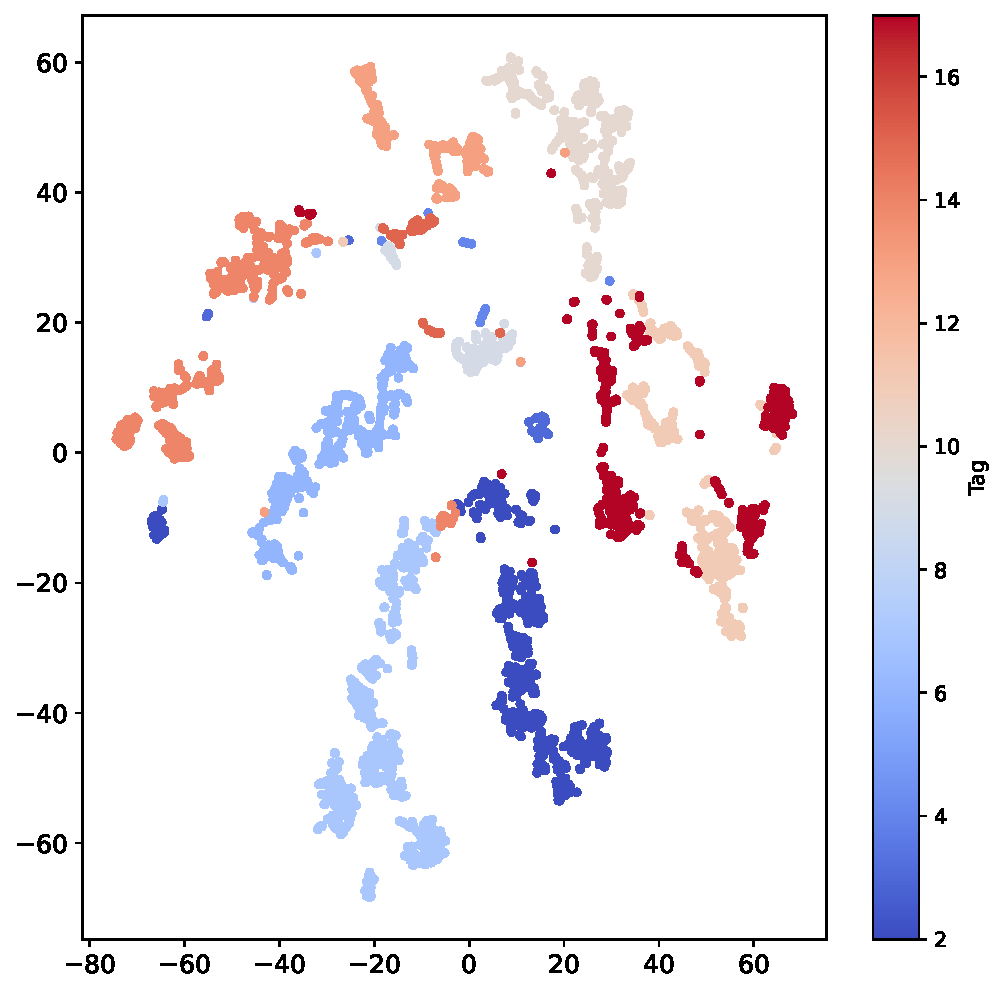
\includegraphics[width=0.5\textwidth]{tsne_2d.pdf}
  \caption{tSNE sample image}\label{fig:tsne}
\end{figure}

\subsection{Subsection Example}
This is a subsection example.

\subsubsection{Subsubsection Example}
This is a subsubsection example.



\chapter{Related Works}
This chapter provides a sample structure for related works and literature review.
A table is attached as \Cref{table:performance}.

\begin{table}[htbp]
  \centering
  \begin{tabular}{lcc}
    \hline
    Model & RMSE & MAE \\
    \hline
    Linear Regression & 12.4 & 9.7 \\
    Random Forest     & 10.8 & 8.5 \\
    LSTM              &  8.2 & 6.9 \\
    \hline
  \end{tabular}
  \caption{Comparison of predictive model performance}\label{table:performance}
\end{table}

% --------------------------------------------------------------------
% BACK MATTER
% --------------------------------------------------------------------
\backmatter

\bibliographystyle{cas-model2-names} % bst downloaded from https://www.elsevier.com/researcher/author/policies-and-guidelines/latex-instructions
\bibliography{refs}

\begin{acknowledgments}
This thesis would not have been possible without the support and encouragement of many people.  
I am deeply grateful for their contributions.  
\end{acknowledgments}


\end{document}
